UAVs are becoming useful partners in many situations and their low cost, compactness and versatility, has grown the researches interest in a lot of different applications. For instance the effectiveness of UAVs usage was assessed in different application problems, such as crop disease detection \cite{cropdisdect}, complex environment exploration \cite{complenvexp}, fire monitoring, detection and fighting \cite{FireUAV}.\\
In all of the possible different applications, different control strategies are being used and refined in the years. One of the most investigated problem is target localization and following. This can be done using GPS position of both target and follower, but this solution remains too environmental restrictive, since in some situations, as for indoor application where satellites have poor precision or can even completely fail \cite{GPS-denied}, it is not suitable.\\
Nowadays most of the solutions to overcome this environment-related problems, are vision-based \cite{visualinertialrev}. They can rely on the flexibility in target changing and are already embedded in most of the commercial drones, for video shooting. The problems with these solutions is that they are based on computationally expensive image processing algorithm, and they have high power consumptions. Since computational limitation and battery duration are two well known UAVs problems \cite{UAVlimits}, the needing of more "light" solutions is researched.
A category of localization technology that shows high performance with a low power consumption and low computational effort, is the Radio Frequency (RF) based. These solutions make use of metrics such as Time of Arrival (ToA), Time Difference of Arrival (TDoA), Angle of Arrival (AoA), and Received Signal Strength (RSS), to perform localization. Some example of the technologies that can provides these measurements are Wi-Fi, Bluetooth, Ultra-Wideband (UWB), Zigbee, Radio Frequency Identification Devices (RFID), Long-Range Radio (LoRA), and cellular networks \cite{radiofreqloc}. Among all these possible solutions, UWB presents some unique characteristics like low-cost, low latency, low energy consumption, and centimeter-level accuracy. Moreover, as for the other RF-based application, UWB localization does not suffer from low-visibility conditions. For these reasons, many researchers in the field have studied localization, following and many other robotic applications using UWB-based architectures.\\
For instance, \citet{elderlycare} have developed an assisted PDoA positioning method for elderly care. They have developed a method to get rid of the Non-Line-Of-Sight (NLOS) error for elderly localization in elder-care structures. The method start with a first coarse localization with pure PDoA measures, subsequently refined by finding the actual antennas that are in Line-Of-Sight, providing an eventual NLOS compensation, and a final convex regression estimation.\\
A work more focused on following, is the one of \citet{Uwbbasedsol}, in which they have proposed a UWB-based solution, that fuse with a Kalman filter, ranging measures coming from three UWB anchors, deployed on the drone in a triangular shape to avoid position ambiguities, with a target which is assumed to move with a linear motion model. More specifically, they have shown that baseline length has an inversely proportional relationship with localization accuracy and with an Hardware-in-The-Loop simulation, and even with preliminary experimental-results on a commercial drone, they have demonstrate the functionality of the proposed following solution. In \cite{sidebyside} the authors present a side-by-side following method for a differential drive robot. They use PDoA measures developing a recursive least square parameter adaptation algorithm (RLS-PAA), which performs a control parameter regression while the target person is walking. On experimental test, considering a safe side distance of $0.5$ meters, they have achieved a true person-robot distance beyond $0.430$ meters for a circle trajectory and $0.482$ meters for a square trajectory, respectively, following quite well the shape of the target path.\\
To our knowledge, not a lot of work that make use of both TDoA and PDoA for localization, are present in the literature, with a complete absence of following application involving these measures. An example could be the optimization-based position algorithm presented by \citet{tdoapdoa_optim}. The proposed method starts with an initial location estimate, obtained by optimizing a TDOA cost function (considering a set of N measures obtained by N anchors deployed in the environment). Next, a PDOA, or a hybrid TDOA-PDOA cost function, is optimized using a particle swarm optimizer to obtain the final location estimate. This procedure has been proven to be effective in improving localization performance relative to pure TDOA methods.\\

Differently from the reviewed target following work \cite{Uwbbasedsol,sidebyside}, our work has the aim of asserting if TDoA and PDoA measures (from where range and AoA are calculated respectively), can be enough to follow a target with enough accuracy w.r.t. the wanted strategy. Indeed no filtering, except of a PDoA averaging, is primarily performed to calculate the controls. To this end, we used a special kind of Ultra-wideband (UWB) pair of antennas, developed by Qorvo. This kit is composed by a classic single UWB antenna and a double one, with their own Nordic companion board for the firmware. The kit was not developed and commercialized specifically to be compact and to be used on a moving robotic agent. In fact, it has a non negligible weight and encumbrance, that of course impact the overall system performance, both in power consumption and stability. However, since this work has the aim of studying the effectiveness of the TDoA/PDoA-based target following, this is not a problem. Thanks to the presence of an array of two antennas, the double UWB, which is deployed on the robotic agent, calculate both range and AoA w.r.t. the single UWB (i.e. the target). These two quantities are the minimum needed to localize the target w.r.t. the agent local reference frame in polar coordinates. In the proposed architecture, as can be seen in \autoref{INT:fig:drone_photo} the double UWB is mounted on a a compact 250 mm wheelbase UAV, whereas the target UWB could be kept by a human being or mounted on another robotic agent. The main contributions of this work are:
\begin{itemize}
    \item The development of an algorithm for target localization, given ranging and AoA measures;
    \item The development of a Gazebo Software-in-The-Loop simulation to evaluate the proposed following strategy;
    \item The Qorvo DW3 QM33 SDK UWB kit characterization;
    \item The development of a repeatable experimental setup, involving Motion Capture for ground truth, to test the described real system.
\end{itemize}
The rest of the paper is organized as follow: in \autoref{PRB_FORM} we formally introduce the problem, the sensed quantities, and the control law. In \autoref{ARCHIT} the quadcopter architecture, together with a description of the robot used as target and of the used motion capture system is exposed. Following, in \autoref{SIMULATION}, after a brief ROS2 introduction, we describe the simulated model of quadcopter and how it interacts with the simulated sensor, in the simulation environment. The implementation details, are instead exposed in \autoref{IMPLM_DET}, whereas in \autoref{UWB_CHAR} the UWB sensor kit is characterized. In \autoref{RESULTS} the results of both the simulation and the real test, are presented and compared and in \autoref{CONCLUSIONS} some conclusions and future improvements are discussed.

\begin{figure}
    \centering
    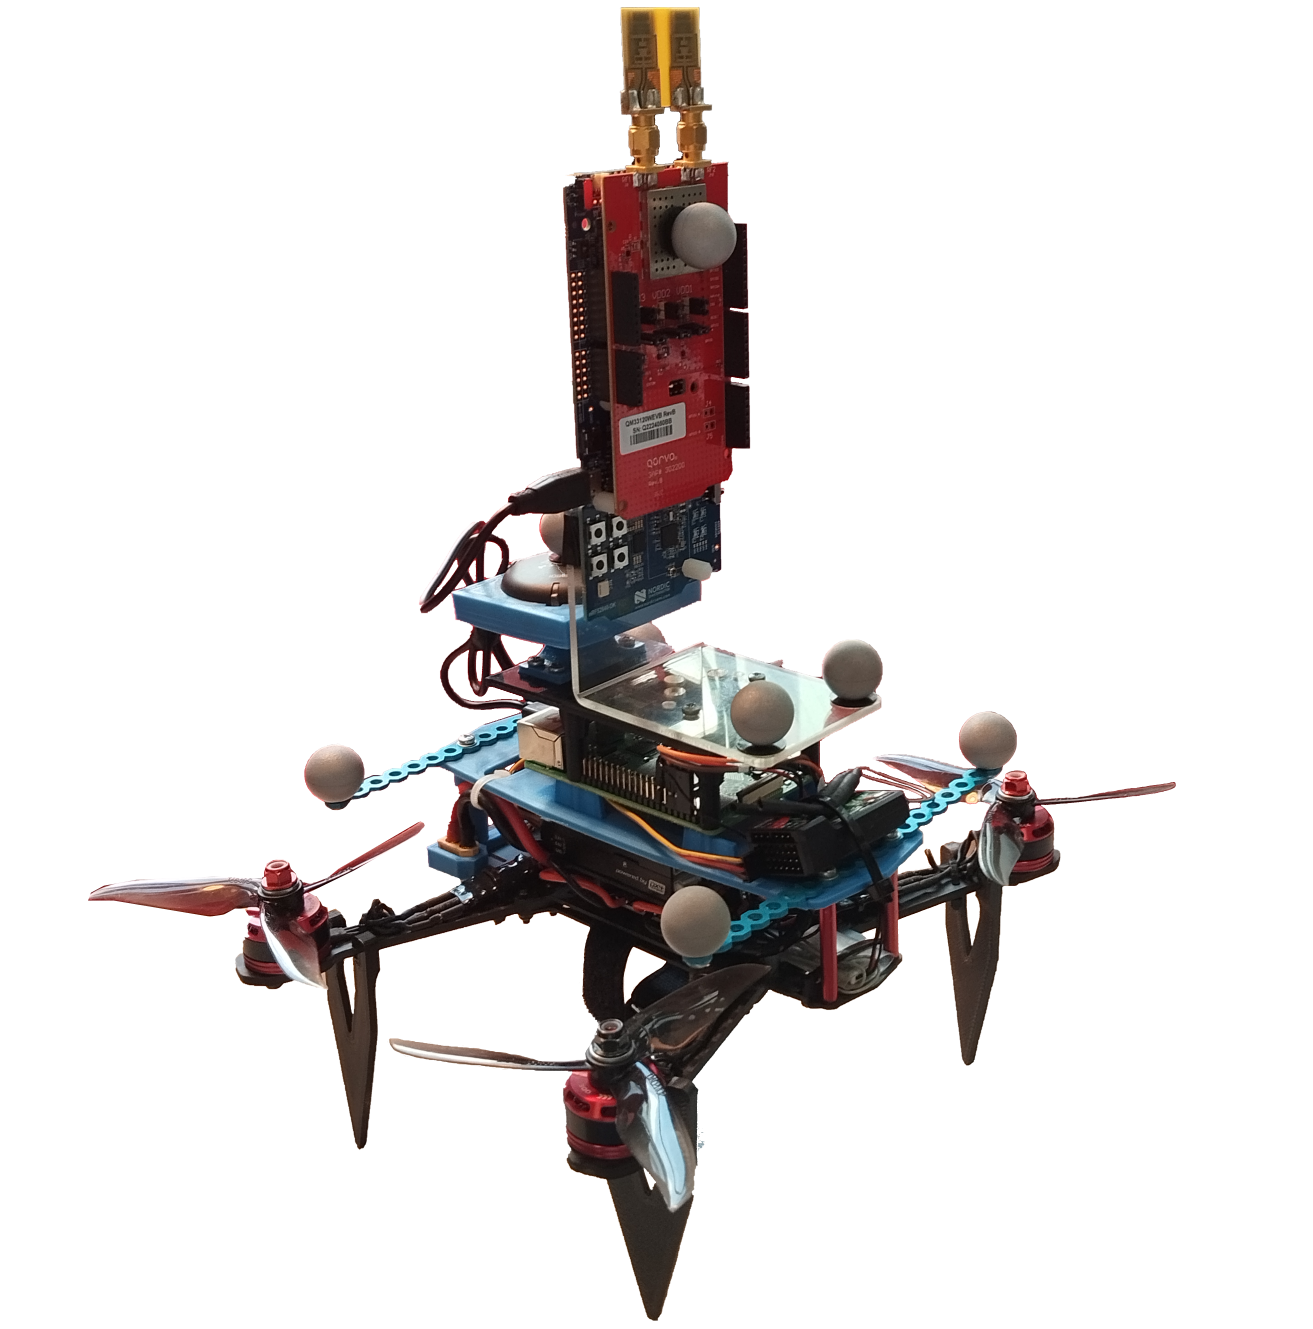
\includegraphics[width=0.4\textwidth]{images/drone_reale_tagliato.png}
    \caption{compact 250mm wheelbase Quadcopter used for the test. It is clearly visible the double antenna on top of the drone, as well as the marker used for the Mocap localization.}
    \label{INT:fig:drone_photo}
\end{figure}


